% Created by tikzDevice version 0.10.1.2 on 2018-05-23 15:20:01
% !TEX encoding = UTF-8 Unicode
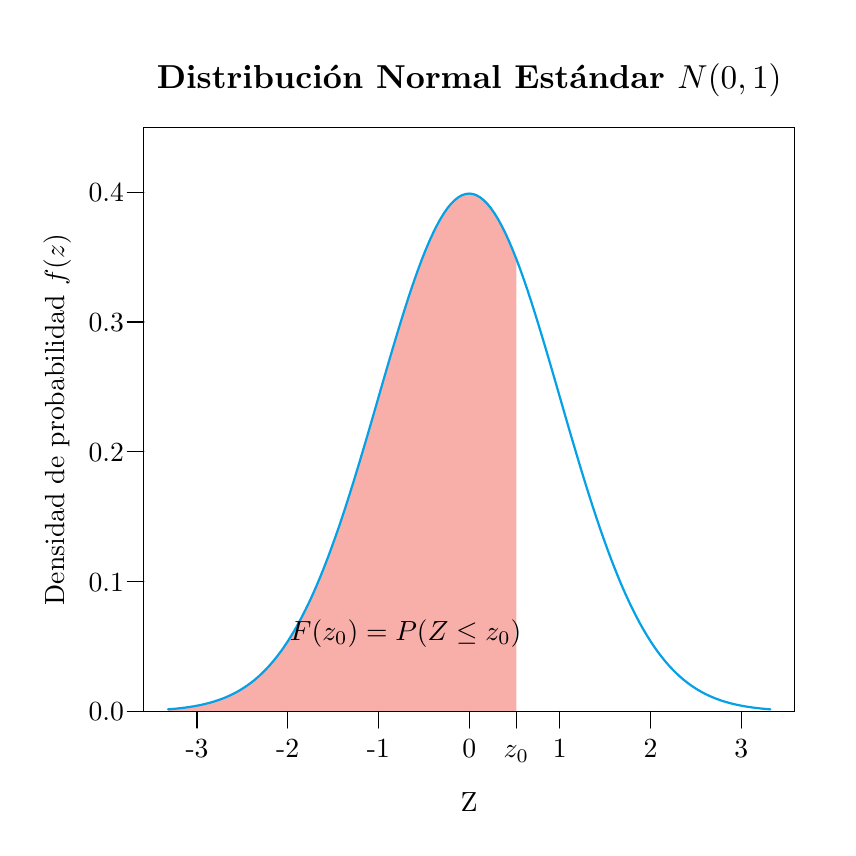
\begin{tikzpicture}[x=1pt,y=1pt]
\definecolor{fillColor}{RGB}{255,255,255}
\path[use as bounding box,fill=fillColor,fill opacity=0.00] (0,0) rectangle (289.08,289.08);
\begin{scope}
\path[clip] (  0.00,  0.00) rectangle (289.08,289.08);
\definecolor{drawColor}{RGB}{0,0,0}

\path[draw=drawColor,line width= 0.4pt,line join=round,line cap=round] ( 61.20, 42.00) -- (257.88, 42.00);

\path[draw=drawColor,line width= 0.4pt,line join=round,line cap=round] ( 61.20, 42.00) -- ( 61.20, 36.00);

\path[draw=drawColor,line width= 0.4pt,line join=round,line cap=round] ( 93.98, 42.00) -- ( 93.98, 36.00);

\path[draw=drawColor,line width= 0.4pt,line join=round,line cap=round] (126.76, 42.00) -- (126.76, 36.00);

\path[draw=drawColor,line width= 0.4pt,line join=round,line cap=round] (159.54, 42.00) -- (159.54, 36.00);

\path[draw=drawColor,line width= 0.4pt,line join=round,line cap=round] (192.32, 42.00) -- (192.32, 36.00);

\path[draw=drawColor,line width= 0.4pt,line join=round,line cap=round] (225.10, 42.00) -- (225.10, 36.00);

\path[draw=drawColor,line width= 0.4pt,line join=round,line cap=round] (257.88, 42.00) -- (257.88, 36.00);

\node[text=drawColor,anchor=base,inner sep=0pt, outer sep=0pt, scale=  1.00] at ( 61.20, 25.20) {-3};

\node[text=drawColor,anchor=base,inner sep=0pt, outer sep=0pt, scale=  1.00] at ( 93.98, 25.20) {-2};

\node[text=drawColor,anchor=base,inner sep=0pt, outer sep=0pt, scale=  1.00] at (126.76, 25.20) {-1};

\node[text=drawColor,anchor=base,inner sep=0pt, outer sep=0pt, scale=  1.00] at (159.54, 25.20) {0};

\node[text=drawColor,anchor=base,inner sep=0pt, outer sep=0pt, scale=  1.00] at (192.32, 25.20) {1};

\node[text=drawColor,anchor=base,inner sep=0pt, outer sep=0pt, scale=  1.00] at (225.10, 25.20) {2};

\node[text=drawColor,anchor=base,inner sep=0pt, outer sep=0pt, scale=  1.00] at (257.88, 25.20) {3};

\path[draw=drawColor,line width= 0.4pt,line join=round,line cap=round] ( 42.00, 42.00) -- ( 42.00,229.63);

\path[draw=drawColor,line width= 0.4pt,line join=round,line cap=round] ( 42.00, 42.00) -- ( 36.00, 42.00);

\path[draw=drawColor,line width= 0.4pt,line join=round,line cap=round] ( 42.00, 88.91) -- ( 36.00, 88.91);

\path[draw=drawColor,line width= 0.4pt,line join=round,line cap=round] ( 42.00,135.81) -- ( 36.00,135.81);

\path[draw=drawColor,line width= 0.4pt,line join=round,line cap=round] ( 42.00,182.72) -- ( 36.00,182.72);

\path[draw=drawColor,line width= 0.4pt,line join=round,line cap=round] ( 42.00,229.63) -- ( 36.00,229.63);

\node[text=drawColor,anchor=base east,inner sep=0pt, outer sep=0pt, scale=  1.00] at ( 34.80, 38.56) {0.0};

\node[text=drawColor,anchor=base east,inner sep=0pt, outer sep=0pt, scale=  1.00] at ( 34.80, 85.46) {0.1};

\node[text=drawColor,anchor=base east,inner sep=0pt, outer sep=0pt, scale=  1.00] at ( 34.80,132.37) {0.2};

\node[text=drawColor,anchor=base east,inner sep=0pt, outer sep=0pt, scale=  1.00] at ( 34.80,179.28) {0.3};

\node[text=drawColor,anchor=base east,inner sep=0pt, outer sep=0pt, scale=  1.00] at ( 34.80,226.18) {0.4};

\path[draw=drawColor,line width= 0.4pt,line join=round,line cap=round] ( 42.00, 42.00) --
	(277.08, 42.00) --
	(277.08,253.08) --
	( 42.00,253.08) --
	( 42.00, 42.00);
\end{scope}
\begin{scope}
\path[clip] (  0.00,  0.00) rectangle (289.08,289.08);
\definecolor{drawColor}{RGB}{0,0,0}

\node[text=drawColor,anchor=base,inner sep=0pt, outer sep=0pt, scale=  1.20] at (159.54,266.94) {\bfseries Distribución Normal Estándar $N(0,1)$};

\node[text=drawColor,anchor=base,inner sep=0pt, outer sep=0pt, scale=  1.00] at (159.54,  6.00) {Z};

\node[text=drawColor,rotate= 90.00,anchor=base,inner sep=0pt, outer sep=0pt, scale=  1.00] at ( 13.20,147.54) {Densidad de probabilidad $f(z)$};
\end{scope}
\begin{scope}
\path[clip] (  0.00,  0.00) rectangle (289.08,289.08);
\definecolor{drawColor}{RGB}{0,0,0}

\path[draw=drawColor,line width= 0.4pt,line join=round,line cap=round] (176.59, 42.00) -- (176.59, 42.00);

\path[draw=drawColor,line width= 0.4pt,line join=round,line cap=round] (176.59, 42.00) -- (176.59, 36.00);

\node[text=drawColor,anchor=base,inner sep=0pt, outer sep=0pt, scale=  1.00] at (176.59, 25.20) {$z_0$};
\end{scope}
\begin{scope}
\path[clip] ( 42.00, 42.00) rectangle (277.08,253.08);
\definecolor{fillColor}{RGB}{238,50,36}

\path[fill=fillColor,fill opacity=0.39] ( 50.71, 42.00) --
	( 50.71, 42.76) --
	( 52.02, 42.86) --
	( 53.33, 42.98) --
	( 54.64, 43.12) --
	( 55.95, 43.27) --
	( 57.26, 43.44) --
	( 58.57, 43.63) --
	( 59.89, 43.84) --
	( 61.20, 44.08) --
	( 62.51, 44.34) --
	( 63.82, 44.63) --
	( 65.13, 44.96) --
	( 66.44, 45.32) --
	( 67.75, 45.71) --
	( 69.06, 46.15) --
	( 70.38, 46.63) --
	( 71.69, 47.16) --
	( 73.00, 47.74) --
	( 74.31, 48.37) --
	( 75.62, 49.06) --
	( 76.93, 49.82) --
	( 78.24, 50.64) --
	( 79.55, 51.54) --
	( 80.87, 52.50) --
	( 82.18, 53.55) --
	( 83.49, 54.69) --
	( 84.80, 55.91) --
	( 86.11, 57.23) --
	( 87.42, 58.64) --
	( 88.73, 60.16) --
	( 90.04, 61.78) --
	( 91.36, 63.51) --
	( 92.67, 65.36) --
	( 93.98, 67.33) --
	( 95.29, 69.41) --
	( 96.60, 71.62) --
	( 97.91, 73.96) --
	( 99.22, 76.43) --
	(100.53, 79.03) --
	(101.85, 81.77) --
	(103.16, 84.63) --
	(104.47, 87.63) --
	(105.78, 90.76) --
	(107.09, 94.03) --
	(108.40, 97.42) --
	(109.71,100.95) --
	(111.02,104.59) --
	(112.34,108.35) --
	(113.65,112.23) --
	(114.96,116.22) --
	(116.27,120.30) --
	(117.58,124.48) --
	(118.89,128.75) --
	(120.20,133.09) --
	(121.51,137.49) --
	(122.83,141.94) --
	(124.14,146.44) --
	(125.45,150.96) --
	(126.76,155.50) --
	(128.07,160.04) --
	(129.38,164.56) --
	(130.69,169.05) --
	(132.00,173.50) --
	(133.32,177.88) --
	(134.63,182.19) --
	(135.94,186.40) --
	(137.25,190.50) --
	(138.56,194.48) --
	(139.87,198.30) --
	(141.18,201.97) --
	(142.49,205.47) --
	(143.81,208.77) --
	(145.12,211.87) --
	(146.43,214.74) --
	(147.74,217.39) --
	(149.05,219.79) --
	(150.36,221.94) --
	(151.67,223.82) --
	(152.98,225.43) --
	(154.30,226.75) --
	(155.61,227.79) --
	(156.92,228.53) --
	(158.23,228.98) --
	(159.54,229.13) --
	(160.85,228.98) --
	(162.16,228.53) --
	(163.47,227.79) --
	(164.78,226.75) --
	(166.10,225.43) --
	(167.41,223.82) --
	(168.72,221.94) --
	(170.03,219.79) --
	(171.34,217.39) --
	(172.65,214.74) --
	(173.96,211.87) --
	(175.27,208.77) --
	(176.59,205.47) --
	(176.59, 42.00) --
	cycle;
\definecolor{drawColor}{RGB}{5,161,230}

\path[draw=drawColor,line width= 0.8pt,line join=round,line cap=round] ( 50.71, 42.76) --
	( 52.02, 42.86) --
	( 53.33, 42.98) --
	( 54.64, 43.12) --
	( 55.95, 43.27) --
	( 57.26, 43.44) --
	( 58.57, 43.63) --
	( 59.89, 43.84) --
	( 61.20, 44.08) --
	( 62.51, 44.34) --
	( 63.82, 44.63) --
	( 65.13, 44.96) --
	( 66.44, 45.32) --
	( 67.75, 45.71) --
	( 69.06, 46.15) --
	( 70.38, 46.63) --
	( 71.69, 47.16) --
	( 73.00, 47.74) --
	( 74.31, 48.37) --
	( 75.62, 49.06) --
	( 76.93, 49.82) --
	( 78.24, 50.64) --
	( 79.55, 51.54) --
	( 80.87, 52.50) --
	( 82.18, 53.55) --
	( 83.49, 54.69) --
	( 84.80, 55.91) --
	( 86.11, 57.23) --
	( 87.42, 58.64) --
	( 88.73, 60.16) --
	( 90.04, 61.78) --
	( 91.36, 63.51) --
	( 92.67, 65.36) --
	( 93.98, 67.33) --
	( 95.29, 69.41) --
	( 96.60, 71.62) --
	( 97.91, 73.96) --
	( 99.22, 76.43) --
	(100.53, 79.03) --
	(101.85, 81.77) --
	(103.16, 84.63) --
	(104.47, 87.63) --
	(105.78, 90.76) --
	(107.09, 94.03) --
	(108.40, 97.42) --
	(109.71,100.95) --
	(111.02,104.59) --
	(112.34,108.35) --
	(113.65,112.23) --
	(114.96,116.22) --
	(116.27,120.30) --
	(117.58,124.48) --
	(118.89,128.75) --
	(120.20,133.09) --
	(121.51,137.49) --
	(122.83,141.94) --
	(124.14,146.44) --
	(125.45,150.96) --
	(126.76,155.50) --
	(128.07,160.04) --
	(129.38,164.56) --
	(130.69,169.05) --
	(132.00,173.50) --
	(133.32,177.88) --
	(134.63,182.19) --
	(135.94,186.40) --
	(137.25,190.50) --
	(138.56,194.48) --
	(139.87,198.30) --
	(141.18,201.97) --
	(142.49,205.47) --
	(143.81,208.77) --
	(145.12,211.87) --
	(146.43,214.74) --
	(147.74,217.39) --
	(149.05,219.79) --
	(150.36,221.94) --
	(151.67,223.82) --
	(152.98,225.43) --
	(154.30,226.75) --
	(155.61,227.79) --
	(156.92,228.53) --
	(158.23,228.98) --
	(159.54,229.13) --
	(160.85,228.98) --
	(162.16,228.53) --
	(163.47,227.79) --
	(164.78,226.75) --
	(166.10,225.43) --
	(167.41,223.82) --
	(168.72,221.94) --
	(170.03,219.79) --
	(171.34,217.39) --
	(172.65,214.74) --
	(173.96,211.87) --
	(175.27,208.77) --
	(176.59,205.47) --
	(177.90,201.97) --
	(179.21,198.30) --
	(180.52,194.48) --
	(181.83,190.50) --
	(183.14,186.40) --
	(184.45,182.19) --
	(185.76,177.88) --
	(187.08,173.50) --
	(188.39,169.05) --
	(189.70,164.56) --
	(191.01,160.04) --
	(192.32,155.50) --
	(193.63,150.96) --
	(194.94,146.44) --
	(196.25,141.94) --
	(197.57,137.49) --
	(198.88,133.09) --
	(200.19,128.75) --
	(201.50,124.48) --
	(202.81,120.30) --
	(204.12,116.22) --
	(205.43,112.23) --
	(206.74,108.35) --
	(208.06,104.59) --
	(209.37,100.95) --
	(210.68, 97.42) --
	(211.99, 94.03) --
	(213.30, 90.76) --
	(214.61, 87.63) --
	(215.92, 84.63) --
	(217.23, 81.77) --
	(218.55, 79.03) --
	(219.86, 76.43) --
	(221.17, 73.96) --
	(222.48, 71.62) --
	(223.79, 69.41) --
	(225.10, 67.33) --
	(226.41, 65.36) --
	(227.72, 63.51) --
	(229.04, 61.78) --
	(230.35, 60.16) --
	(231.66, 58.64) --
	(232.97, 57.23) --
	(234.28, 55.91) --
	(235.59, 54.69) --
	(236.90, 53.55) --
	(238.21, 52.50) --
	(239.53, 51.54) --
	(240.84, 50.64) --
	(242.15, 49.82) --
	(243.46, 49.06) --
	(244.77, 48.37) --
	(246.08, 47.74) --
	(247.39, 47.16) --
	(248.70, 46.63) --
	(250.02, 46.15) --
	(251.33, 45.71) --
	(252.64, 45.32) --
	(253.95, 44.96) --
	(255.26, 44.63) --
	(256.57, 44.34) --
	(257.88, 44.08) --
	(259.19, 43.84) --
	(260.51, 43.63) --
	(261.82, 43.44) --
	(263.13, 43.27) --
	(264.44, 43.12) --
	(265.75, 42.98) --
	(267.06, 42.86) --
	(268.37, 42.76);
\definecolor{drawColor}{RGB}{0,0,0}

\node[text=drawColor,anchor=base,inner sep=0pt, outer sep=0pt, scale=  1.00] at (136.59, 67.64) {$F(z_0)=P(Z\leq z_0)$};
\end{scope}
\begin{scope}
\path[clip] (  0.00,  0.00) rectangle (289.08,289.08);
\definecolor{drawColor}{RGB}{0,0,0}

\path[draw=drawColor,line width= 0.4pt,line join=round,line cap=round] ( 42.00, 42.00) --
	(277.08, 42.00) --
	(277.08,253.08) --
	( 42.00,253.08) --
	( 42.00, 42.00);
\end{scope}
\end{tikzpicture}
